\documentclass{article}

\usepackage[normalem]{ulem}
\usepackage{fancyhdr}
\usepackage[parfill]{parskip}
\usepackage{tikz}
\pagestyle{fancyplain}

\title{Oscillations}
\author{Todd Davies}
\date{\today}

\begin{document}

\rhead{Oscillations}
\lhead{\today}

\maketitle

\section*{What's an oscillation?}
\thispagestyle{empty}
An oscillation is defined as a '\textit{A repetitive back and forth motion}' (an object that oscillates can also be said to vibrate).

\section*{Equations you need to know}
\begin{itemize}
	\item The angular velocity is related to the time period of the oscillation with the following equation:
	\[
		\omega = \frac{2 \pi}{T}
	\]
	Which is of course equal to:
	\[
	 \omega = 2 \pi f
	\]
	\item In simple harmonic motion, displacement can be calculated using the following:
	\[
		x = A \sin (2 \pi ft)
	\]
	or
	\[
		x = A \cos(2 \pi ft)
	\]
	\item The acceleration of a body undergoing simple harmonic motion is proportional to it's displacement from the equlibrium position:
	\[
		a \propto x
	\]
	We can include the constant in the equation to give:
	\[
		a = -(2 \pi f)^{2}x
	\]
	\item The maximum speed of an object undergoing simple harmonic motion can be found using:
	\[
		v_{max} = (2 \pi f)A
	\]
\end{itemize}

\textit{N.b. all equations take radians, not degrees}

The quantities and their respective units are shown in this table:

\begin{center}
	\begin{tabular}{|l|l|l|}
		\hline
			Quantity & Abbreviation & Unit \\ \hline
			Time period & $T$ & Second ($s$) \\ \hline
			Frequency & $f$ & Hertz ($Hz$) \\ \hline
			Acceleration & $a$ & Metres per second squared ($ms^{-2}$) \\ \hline
			Time & $t$ & Seconds($s$) \\ \hline
			Angular velocity & $\omega$ & Radians per second($rad/s$) \\ \hline
			Amplitude & $A$ & Meters ($m$) \\ \hline
			Velocity & $v$ & Meters per second ($ms^{-1}$) \\ \hline
			Displacement & $x$ & Meters ($m$) \\ \hline
	\end{tabular}
\end{center}

\section*{Types of oscillation}
There are two types of oscillation - free and forced.
\subsection*{Free oscillations}
This is when an object is left to vibrate at it's \textit{natural frequency}. The oscillating object is under no external influence (other than the influence that initiated the motion). 

An example of a free oscillation could be when you pluck a violin string. The string oscillates at its natural frequency which produces the note that you hear.
\subsection*{Forced oscillations}
A forced oscillation is when an object moves back and forth under the influence of another driving object.

An example of this is if you wave your hand at somebody. Your arm is driving your hand, but your hand isn't moving at it's natural frequency.

\section*{Describing an oscillation}
Oscillations have maximum velocity at the point where their displacement is zero. At this point, they have minimum acceleration.
Oscillations have maximum acceleration at the point where their displacement is maximum. At this point they have minimum velocity.
The shape of a graph plotting displacement against time is going to be something like:

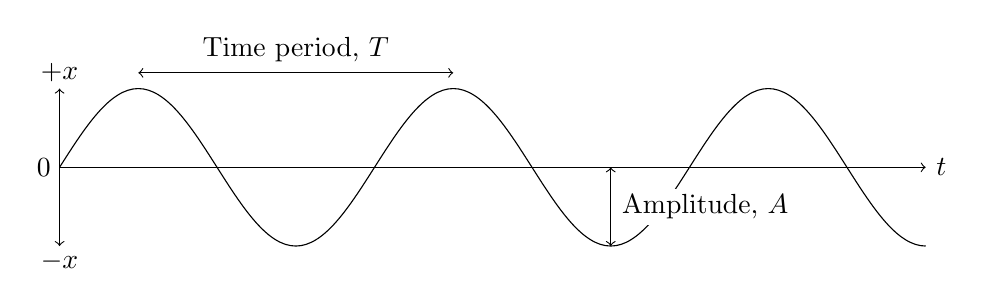
\begin{tikzpicture}
	%curve
		\draw (0.5,0) sin (1.5,1) cos (2.5,0) sin (3.5,-1) cos (4.5,0) sin (5.5,1) cos (6.5,0) sin (7.5,-1) cos (8.5,0) sin (9.5,1) cos (10.5,0) sin (11.5,-1);
	% zero crossing
		\draw[dotted] (0.5,0) -- (11.5,0);
	%axis + labels
		\draw [<->] (0.5,1) -- (0.5,-1);
		\draw [->] (0.5,0) -- (11.5,0);
		\node at (11.7,0) {$t$};
		\node at (0.5,1.2) {$+x$};
		\node at (0.5,-1.2) {$-x$};
		\node at (0.3,0) {$0$};
	%Time period description
		\draw [<->] (1.5,1.2) -- (5.5,1.2);
		\node at (3.5,1.5) {Time period, $T$};
	%Amplitude description
		\draw [<->] (7.5,0) -- (7.5,-1);
		\draw [fill=white,ultra thick,white] (7.6,-0.3) rectangle (9.7,-0.7); %to stop line overlap
		\node at (8.7, -0.5) {Amplitude, $A$};
\end{tikzpicture}

This graph can be described as \textit{sinusoidal}.

\section*{Phase}
As you should know from the G482 module, waves have a phase. The phase of a wave is the point an oscillating mass has reached in it's cycle of oscillation. Phase is measured in degrees or radians. Two waves can have a phase difference, also measured in degrees or radians.

Here is a diagram of two identical waves out of phase by 180 degrees:

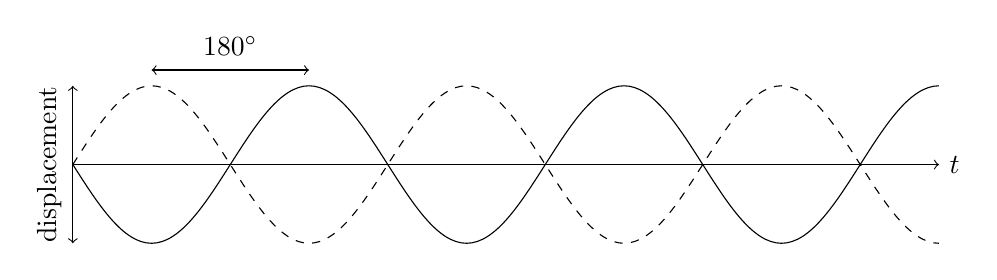
\begin{tikzpicture}
	%curve 1
		\draw[dashed] (0.5,0) sin (1.5,1) cos (2.5,0) sin (3.5,-1) cos (4.5,0) sin (5.5,1) cos (6.5,0) sin (7.5,-1) cos (8.5,0) sin (9.5,1) cos (10.5,0) sin (11.5,-1);
	%curve 2
		\draw (0.5,0) sin (1.5,-1) cos (2.5,0) sin (3.5,1) cos (4.5,0) sin (5.5,-1) cos (6.5,0) sin (7.5,1) cos (8.5,0) sin (9.5,-1) cos (10.5,0) sin (11.5,1);
	% zero crossing
		\draw[dotted] (0.5,0) -- (11.5,0);
	%axis + labels
		\draw [<->] (0.5,1) -- (0.5,-1);
		\draw [->] (0.5,0) -- (11.5,0);
		\node at (11.7,0) {$t$};
		\node[rotate=90] at (0.2,0) {displacement};
	%Phase difference description
		\draw [<->] (1.5,1.2) -- (3.5,1.2);
		\node at (2.5,1.5) {$180^\circ$};
\end{tikzpicture}

\textit{N.b. 180 degrees is equal to $\pi$ radians.}

\section*{Simple harmonic motion (SHM)}
\textbf{Definition: }\textit{A body executes simple harmonic motion if its acceleration is directly proportional to its displacement from its equilibrium position and is always directed towards the equilibrium position.}

Examples of SHM include:
\begin{itemize}
	\item The string of a violin after it has been plucked
	\item The pendulum of a grandfather clock
	\item When a pure sound travels through the air, the molecules in the air vibrate with SHM
	\item The alternating current found in the national grid makes electrons in the wire move with SHM
\end{itemize}

At A-level, only oscillations with one frequency are analysed, however SHM can also apply to objects that have a complicated motion equal to the resultant of many different waves.

\subsection*{The requirements of SHM}
The three requirements of SHM are:
\begin{enumerate}
	\item A mass must oscillate
	\item There must be a position where the mass is in equilibrium
	\item There must be a restoring force that acts to return the mass to equilibrium. This force is proportional to the displacement of the mass from the equilibrium position and is directed towards the equilibrium position.
\end{enumerate}

\subsection*{Changes displacement, velocity and acceleration in SHM}
If you do maths mechanics, then you're in luck for this bit!
We can find the displacement of the mass for a given time using this equation:
\[
	x = A\sin (2 \pi ft)
\]
If we differentiate this, we get:
\[
	\frac{dx}{dt} = v = 2 \pi f A cos(2 \pi f t)
\]
And if we differentiate again, we get:
\[
	\frac{dx^2}{d^2t} = a = - A (2 \pi f)^2 sin(2 \pi f t)
\]

\textit{N.b. We can sub in the equation for displacement into the equation we derived for the acceleration to get $a= -(2 \pi f)^2 x$ which is the equation on the formulae sheet.}

However, that wasn't on the syllabus, but you \textit{do need to know} the following:
\begin{itemize}
	\item Velocity is highest when $x=0$ and lowest (zero) when $x=A$.
	\item Acceleration is the inverse of the velocity (i.e. it's highest when $x=A$ and lowest when $x=0$).
\end{itemize}

\subsection*{Graphical representations of SHM}
If you have a graph of either displacement, velocity or acceleration, you can draw a graph of the other two from the graph you do have. To do this, you plot gradient of the previous graph like so:

\begin{center}
	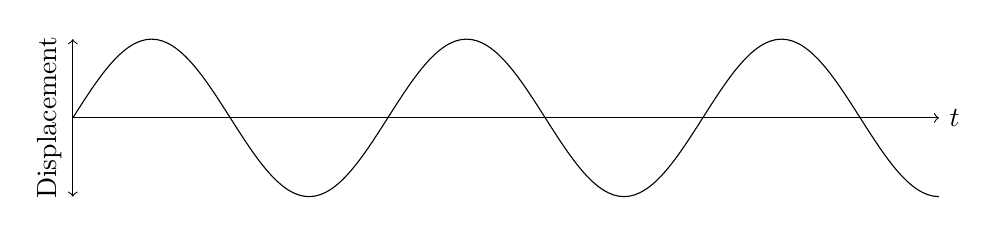
\begin{tikzpicture}
		%curve
			\draw (0.5,0) sin (1.5,1) cos (2.5,0) sin (3.5,-1) cos (4.5,0) sin (5.5,1) cos (6.5,0) sin (7.5,-1) cos (8.5,0) sin (9.5,1) cos (10.5,0) sin (11.5,-1);
		%axis + labels
			\draw [<->] (0.5,1) -- (0.5,-1);
			\draw [->] (0.5,0) -- (11.5,0);
			\node at (11.7,0) {$t$};
			\node[rotate=90] at (0.2,0) {Displacement};
	\end{tikzpicture}

	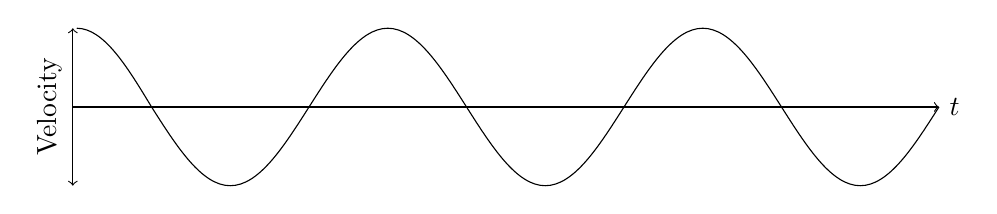
\begin{tikzpicture}
		%curve
			\draw (0.55,1) cos (1.5,0) sin (2.5,-1) cos (3.5,0) sin (4.5,1) cos (5.5,0) sin (6.5,-1) cos (7.5,0) sin (8.5,1) cos (9.5,0) sin (10.5,-1) cos (11.5,0);
		%axis + labels
			\draw [<->] (0.5,1) -- (0.5,-1);
			\draw [->] (0.5,0) -- (11.5,0);
			\node at (11.7,0) {$t$};
			\node[rotate=90] at (0.2,0) {Velocity};
	\end{tikzpicture}

	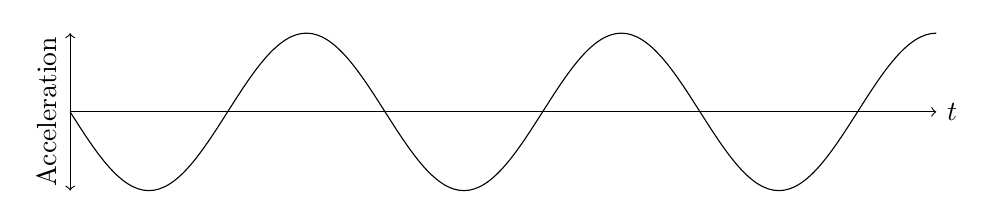
\begin{tikzpicture}
		%curve
			\draw (0.5,0) sin (1.5,-1) cos (2.5,0) sin (3.5,1) cos (4.5,0) sin (5.5,-1) cos (6.5,0) sin (7.5,1) cos (8.5,0) sin (9.5,-1) cos (10.5,0) sin (11.5,1);
		%axis + labels
			\draw [<->] (0.5,1) -- (0.5,-1);
			\draw [->] (0.5,0) -- (11.5,0);
			\node at (11.7,0) {$t$};
			\node[rotate=90] at (0.2,0) {Acceleration};
	\end{tikzpicture}
\end{center}

If you look, you can see that the graph of the velocity is the gradient of the displacement, and the graph of acceleration is the gradient of the velocity. 

By looking at these graphs, we can also deduce that $a \propto -x$.

\subsection*{Angular frequency in SHM}
The angular frequency of an object undergoing SHM relates to the frequency and time period via these equations:
\[
	\omega = 2 \pi f
\]
\[
	\omega = \frac{2 \pi}{T}
\]
\[
	T = \frac{2 \pi}{\omega}
\]
This means you can work out the angular frequency of and object in SHM from a graph of displacement.

\subsection*{The relationship between acceleration and displacement in SHM}
If we were to draw a graph of acceleration on the y axis and displacement on the x axis of an object undergoing SHM, it would look like the following:

\begin{center}
	\begin{tikzpicture}
		%line
			\draw [-] (3,3) -- (-3,-3);
		%axis + labels
			\draw [<->] (4,0) -- (-4,0);
			\draw [->] (0,-4) -- (0,4);
			\node at (0,4.2) {$a$};
			\node at (4.2,0) {$x$};
		%crossing points
			\draw [-, dotted] (3,3) -- (3, -0.5);
			\node at (3.3,-0.3) {$+A$};
			\draw [-, dotted] (-3,-3) -- (-3, 0.5);
			\node at (-2.7,0.3) {$-A$};
		%gradient
			\draw [-, dashed] (2,2) -- (2, -2);
			\draw [-, dashed] (-2,-2) -- (2, -2);
			\node at (2,-2.5) {$\frac{\delta y}{\delta x} = \frac{-(2 \pi ft)^2 \textrm{\sout{$A \sin(2 \pi ft)$}}}{\textrm{\sout{$A \sin(2 \pi ft)$}}}$};
			\node at (2.33,-3.1) {$=-(2 \pi ft)^2 = \textrm{gradient}$};
	\end{tikzpicture}
\end{center}

Notice that the gradient is independent of the amplitude of the graph, which explains why objects in SHM keep a constant frequency even though their amplitude may decrease over time.

\subsection*{Maximum speed of an oscillator}
From the equation 
\[
v_{max} = (2 \pi f)A
\]
We can deduce that:
\[
	v_{max} \propto A
\]
However, since (as we discovered in the previous section), $A$ is independent of $f$, we also find that:
\[
	v_{max} \propto f
\]

\subsection*{Energy changes in SHM}
In SHM, there is a constant change between potential (gravitational, elastic etc) energy and kinetic energy. We can draw graphs of these energies in a system:

\begin{center}
	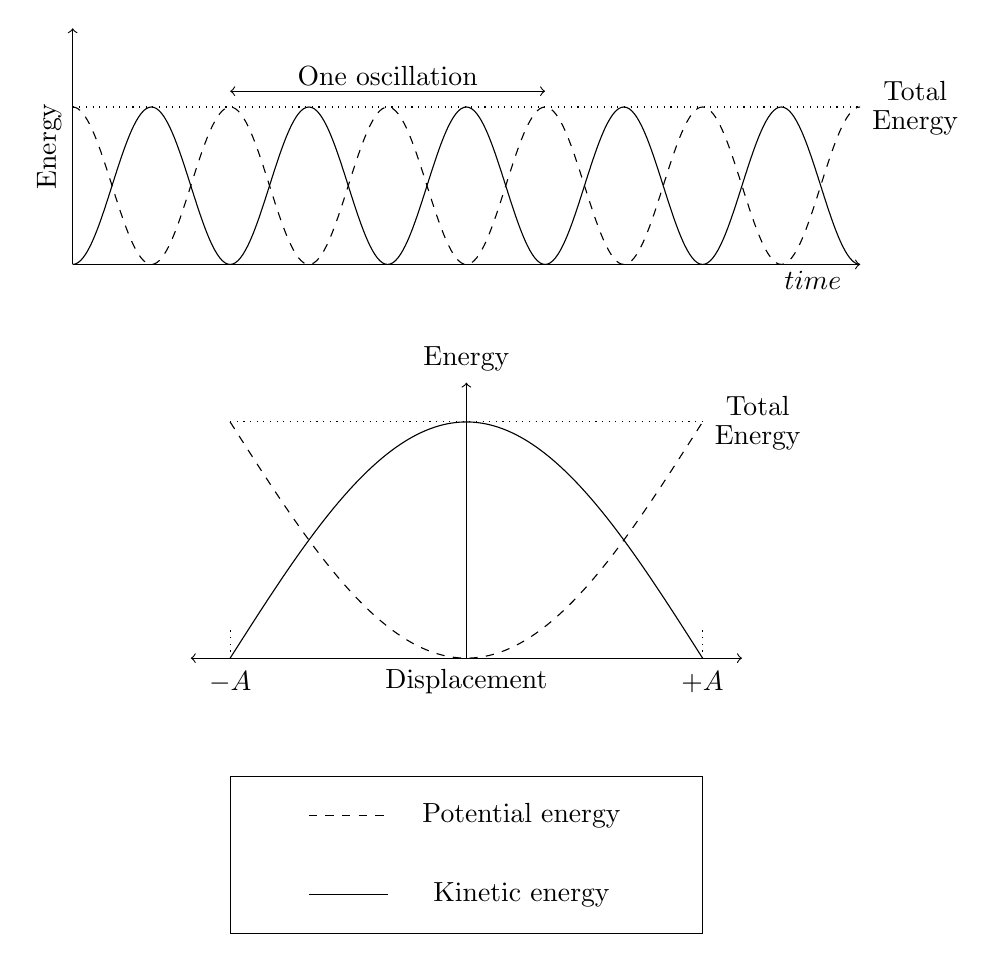
\begin{tikzpicture}
		%Graph 1
			%PE
				\draw[dashed] (1.5,2) cos (2,1) sin (2.5,0) cos (3,1) sin (3.5,2) cos (4,1) sin (4.5,0) cos (5,1) sin (5.5,2) cos (6,1) sin (6.5,0) cos (7,1) sin (7.5,2) cos (8,1) sin (8.5,0) cos (9,1) sin (9.5,2) cos (10,1) sin (10.5,0) cos (11,1) sin (11.5,2);
			%KE
			\draw (1.5,0) cos (2,1) sin (2.5,2) cos (3,1) sin (3.5,0) cos (4,1) sin (4.5,2) cos (5,1) sin (5.5,0) cos (6,1) sin (6.5,2) cos (7,1) sin (7.5,0) cos (8,1) sin (8.5,2) cos (9,1) sin (9.5,0) cos (10,1) sin (10.5,2) cos (11,1) sin (11.5,0);
			%axis + labels
				\draw [->] (1.5,0) -- (1.5,3);
				\draw [->] (1.5,0) -- (11.5,0);
				\node at (10.9,-0.2) {$time$};
				\node[rotate=90] at (1.2,1.5) {Energy};
			%total energy label
				\draw[thin, dotted] (1.5, 2) -- (11.5, 2);
				\node at (12.2, 2.2) {Total};
				\node at (12.2, 1.8) {Energy};
			%one oscillation
				\draw[<->] (3.5, 2.2) -- (7.5, 2.2);
				\node at (5.5, 2.4) {One oscillation};
		%Graph 2
			%PE
				\draw[dashed] (3.5,-2) sin (6.5,-5) cos (9.5,-2);
			%KE
				\draw (3.5,-5) sin (6.5,-2) cos (9.5,-5);
			%axis + labels
				\draw [->] (6.5,-5) -- (6.5,-1.5);
				\draw [<->] (3,-5) -- (10,-5);
				\node at (6.5,-5.3) {Displacement};
				\node at (6.5,-1.2) {Energy};
			%amplitude
				\draw[dotted] (3.5,-5) -- (3.5,-4.6);
				\node at (3.5,-5.3) {$-A$};
				\draw[dotted] (9.5,-5) -- (9.5,-4.6);
				\node at (9.5,-5.3) {$+A$};
			%total energy
				\draw[dotted] (3.5,-2) -- (9.5,-2);
				\node at (10.2, -1.8) {Total};
				\node at (10.2, -2.2) {Energy};
		%Labels
			%PE label
				\draw[dashed] (4.5, -7) -- (5.5, -7);
				\node at (7.2, -7) {Potential energy};
			%KE label
				\draw (4.5, -8) -- (5.5, -8);
				\node at (7.2, -8) {Kinetic energy};
			%label box
				\draw (3.5, -6.5) rectangle (9.5, -8.5);
	\end{tikzpicture}
\end{center}
These graphs show that:
\begin{itemize}
	\item Kinetic energy is maximum when the displacement is equal to zero.
	\item Potential energy is maximum when the displacement is equal to the amplitude of the motion.
	\item At any point, $KE + PE = $\textit{ total energy}
\end{itemize}

\section*{Damped oscillations}
The amplitude of a damped oscillation decreases exponentially with time. This means that is loses lots of energy at first, but takes a long time to stop completely.

Damping is achieved by introducing a frictional force into a mechanical oscillating system. By adding this force, energy is constantly removed from the system, and so the amplitude and maximum speed of the oscillation decrease.

\section*{Resonance}
Resonance is a phenomena where if the frequency of the driving oscillation matches the natural frequency of the object being driven, then the amplitude of the driven object increases exponentially.

For resonance to occur, the system must be capable of moving freely. We also need a driving force. The following statements apply to a system in resonance:
\begin{itemize}
	\item Natural frequency = driving frequency
	\item Amplitude is maximum
	\item Driven system absorbs the greatest possible energy from the driver
\end{itemize}

We can employ damping to reduce the effects of resonance. For example in skyscrapers, damping of the foundations of the building can save the building from collapse in the event of an earthquake.

Resonance can also be useful. Microwaves make water molecules vibrate at their natural frequency and so give them kinetic energy, which heats up the food they are in.
\end{document}